\section{Results}
\label{sec:results}
\subsection{Reference-compatible execution provides complete-service value}
Figure~\ref{fig:service} shows every fixed target-only comparison for the three Linux deployments. LOCAL-packed D4 reduces resident service relative to all four M implementations. Against the fastest measured fixed M, the reductions are 17.21\% for Qwen3-8B, 25.54\% for Qwen3-14B and 11.52\% for Llama-8B. The corresponding average request times change from 2.6898 to 2.2269\,s, 4.6022 to 3.4268\,s and 2.8515 to 2.5230\,s. The adjusted intervals support the direction of each registered M comparison.

\begin{figure*}[t]
\centering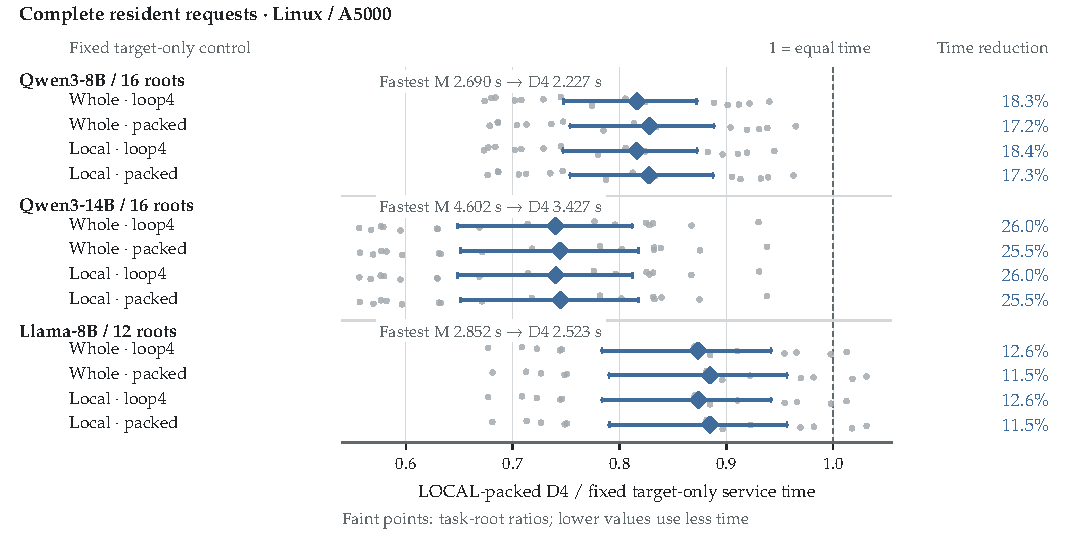
\includegraphics[width=\textwidth]{figures/service_controls.pdf}
\caption{Linux/A5000 resident service. Faint points show all task-root ratios. Each diamond compares LOCAL-packed D4 (draft prefill UB4, $k=3$) with a fixed target-only M; segments are 99\% paired-root intervals from the five-contrast family (the four M comparisons shown here and the W-L4-D4 comparison). Headers give fastest fixed M and D4 mean times. Qwen panels share 16 tasks; Llama has 12. Deployments are analyzed separately. Table~S1 reports all six arm means.}
\label{fig:service}
\end{figure*}

The 14B deployment also retains the benefit outside the internal service timer. The actual measured-request burst totals 294.632\,s for its strongest fixed M and 219.405\,s for LOCAL-packed D4, a 25.53\% reduction. Complete native-worker totals, including integrity checks, loading, primers and the request strings, change from 662.546 to 594.559\,s, a 10.26\% reduction. For Llama, resident requests benefit, while the recorded process-level total favors M for this short worker workload. Table~S2 reports resident and full-worker costs separately.

The Windows practical panel originally selected 16 task roots and retained all four target-only controls. LOCAL-packed D4 reduces resident service by 29.11\%, actual request-burst time by 29.09\% and worker-wall time by 26.00\%. Its complete phase account locates the savings primarily in continuation/verification. Supplement~S2 gives the absolute times and disjoint cost balance. The Linux Qwen panels reuse the Windows task records, while numerical references, measurements and deployment lifecycles are established separately.

Compatible target verification saves enough target work to cover draft work in these deployments. This gain belongs to the reference-compatible application, which whole-graph execution also supports. The balanced studies resolve the incremental effects of the two implementation choices.

\subsection{Balanced studies separate the sources of improvement}
\label{sec:factors}
The four-D4 factorial experiments hold the model, draft policy and transaction width fixed, then cross W/L cuts with loop4/packing. Every arm is remeasured in the same panel. Figure~\ref{fig:factorial} includes the root-level ratios and all four direct effects for both Qwen scales; the fifth member of the simultaneous-inference family is the root-level interaction reported in Supplement~S3.

\begin{figure*}[t]
\centering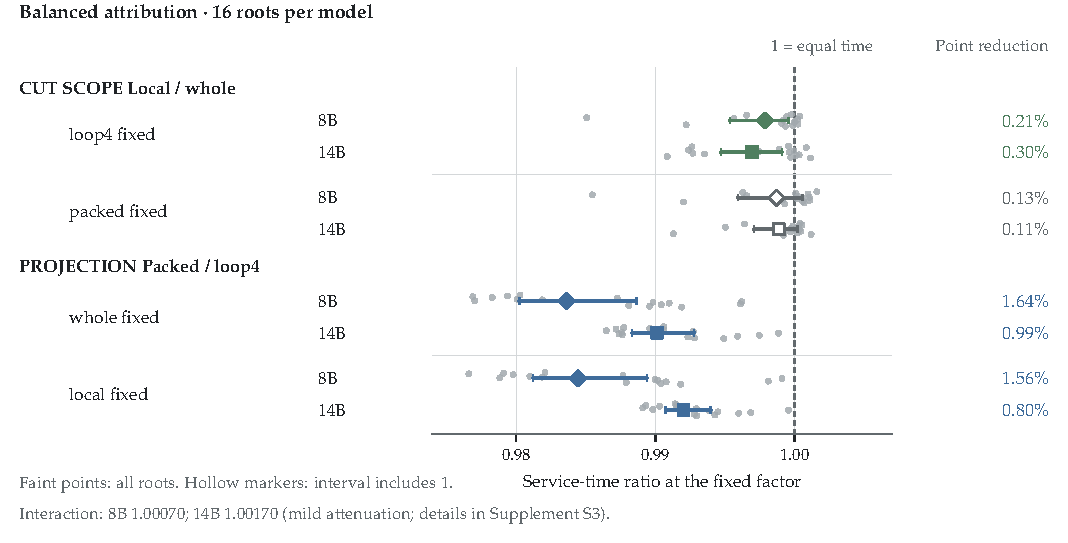
\includegraphics[width=\textwidth]{figures/factorial.pdf}
\caption{Balanced D4 attribution. Faint points show all 16 root ratios. Diamonds (8B) and squares (14B) mark complete-service total ratios; segments are 99\% adjusted intervals. Hollow, neutral markers identify intervals that include 1. The two sections isolate cut scope and projection. Table~S3 lists the fixed effects; Supplement~S3 defines the equal-root interaction.}
\label{fig:factorial}
\end{figure*}

At 8B, packing reduces service by 1.64\% with W and 1.56\% with L; at 14B, it saves 0.99\% and 0.80\%. Backend-loop4 already moves the simple loop out of the graph, so these comparisons measure the remaining packing increment.

At fixed loop4, local cuts save 0.21\% and 0.30\% for 8B and 14B. At fixed packing, the point reductions are 0.13\% and 0.11\%, with intervals containing 1. The interactions, 1.000696 and 1.001703, indicate mild attenuation when the two optimizations are combined.

The physical execution explains the scale of the cut effect. In the 8B factorial, 20 of 2,224 logical verification cycles require an extra whole-graph boundary split, approximately 0.899\%. LOCAL executes 2,224 four-row graphs and W executes 2,244 verification graphs, with the same number of target rows and the same prefill-width distribution. Local grouping avoids repeated graph work at those boundaries; most calls already have compatible geometry. The native observer places wide packing in prefill, not in four-row verification. This phase distinction explains where packing can contribute at $k=3$.

Packing organizes independent arithmetic groups, while local cuts preserve outer parallelism when a physical boundary divides a call. A deployment selects the implementations; per-call planning supplies their compatible groups.

\subsection{Typed grouping extends the method to 32B mixed quantization}
\label{sec:q4result}
The 32B deployment contains 385 Q4\_K, 65 Q6\_K and 257 F32 tensors. Its REF1 recipe is a typed extension: it retains scalar-column arithmetic for the mixed quantized projections and exposes independent columns as channels. All six paths pass finite vector/state checks before the four-root descriptive timing panel. The candidates share C1024, F16 KV, reserve 32 and a CUDA-Graphs-disabled policy. Transformer and output layers are GPU offloaded, with the standard CPU-mapped input embedding.

\begin{figure}[t]
\centering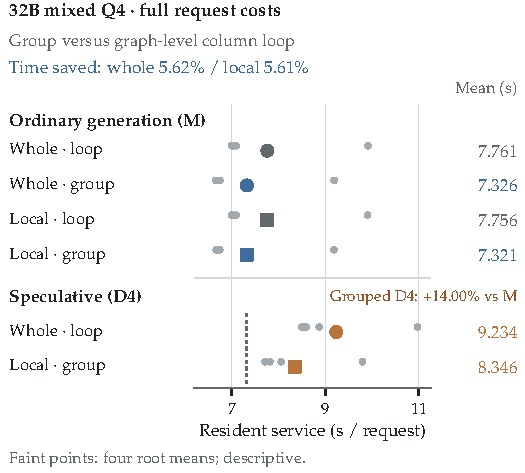
\includegraphics[width=\columnwidth]{figures/mixed_q4.pdf}
\caption{All six 32B mixed-Q4 paths. Markers and numbers give mean service; faint points are four exposed-root means over four rounds. Circles/squares distinguish whole/local scope. The loop control is graph-level scalar-column execution. Grouped D4 uses 14.00\% more time than the fastest M (dotted reference). Table~S4 reports complete costs.}
\label{fig:q4}
\end{figure}

Grouping reduces ordinary service from 124.183 to 117.208\,s with W fixed (5.62\%), and from 124.100 to 117.144\,s with L fixed (5.61\%), over 16 requests per arm. Both comparisons improve in all 16 matched root/round pairs. Worker totals fall by 3.98\% and 4.56\%, and caller totals by 3.85\% and 3.81\%, respectively. The grouped implementation retains scalar-column arithmetic while replacing separate column graphs and concatenation with one operation over independent channels.

Figure~\ref{fig:q4} identifies target-only grouped execution as the appropriate measured application choice. The grouped D4 path improves on the graph-loop D4 path, but takes 14.00\% more resident time than the fastest M. The ordinary-generation comparison fixes cut scope and excludes draft work, isolating the measured grouping package. A subsequent operand-level comparison with a backend-internal loop is reported in Supplement~S3.



\subsection{Physical geometry determines the value of local cuts}
The final Vulkan interface supports actual C1024 and C4096 allocations, the original prompt producer and known-query appends of 2, 4 and 32 rows. Figure~\ref{fig:vulkan} retains both within-bucket and crossing cases. In the six crossing coordinates, LOCAL reduces append time by 20.34\%--44.68\% relative to W. The paired inside controls are within approximately 0.43\%--3.74\% in the other direction.

\begin{figure}[t]
\centering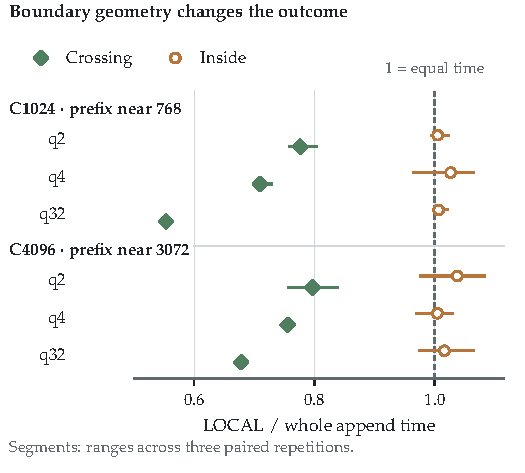
\includegraphics[width=\columnwidth]{figures/vulkan_geometry.pdf}
\caption{Vulkan append geometry. Filled diamonds denote crossings, hollow circles the inside controls, and the dashed line equal time. Segments show the minimum and maximum of the three observed paired ratios, not a population interval. Crossings split one row from the remainder. C1024 and C4096 jointly change capacity and active-prefix region.}
\label{fig:vulkan}
\end{figure}

Split geometry determines the work preserved by a local cut. Earlier q32 experiments used $16+16$ whole-graph splits and included cases favoring W; the final interface probes a $1+31$ split, one row before a physical boundary. The earlier full CUDA width/geometry matrix is reproduced in Supplement~S5. Its twelve fixed coordinates include cases where packing regresses, including Qwen crossing widths. The historical Vulkan cells are retained in Supplementary Fig.~S2. Natural alignment and whole-graph rechunking can make the schedules nearly coincide. Local grouping provides its benefit where it avoids fragmentation of the surrounding graph.

Vulkan executes two-query verification within the reference contract. In a separate resident mechanism window, LOCAL executes 578 occupied two-row target graphs for 1,156 rows, versus 1,156 scalar graphs in the earlier resident speculative path. Ordinary M executes 992 graphs for 992 rows. Batching reduces graph invocations while speculation changes the amount of target work. The complete pilot cost, including draft work, favors M in that deployment. The earlier natural-prefix AUTO panels on both RTX and B570 did not establish a service benefit over fixed policies; the strong whole-graph rechunk control can absorb much of the append-only gain. Supplement~S5 retains those separate negative controls and their lifecycles.

\subsection{Eight-row execution improves equal work; live width changes work}
\label{sec:width}
The $q=8$ implementation retains Q8\_0 weights and the arithmetic reference, extending the transaction to $k=7$ with candidate output reserve 8 for both widths. The width is physical: LOCAL can execute eight verification positions, while W splits according to actual extents. Original requested rows, pending/correction/bonus state, trim frontier and terminal handling are qualified against the independent reference.

\begin{figure*}[t]
\centering
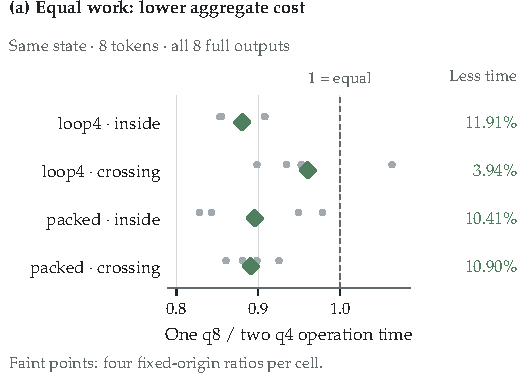
\includegraphics[width=.493\textwidth]{figures/width_equal.pdf}\hfill
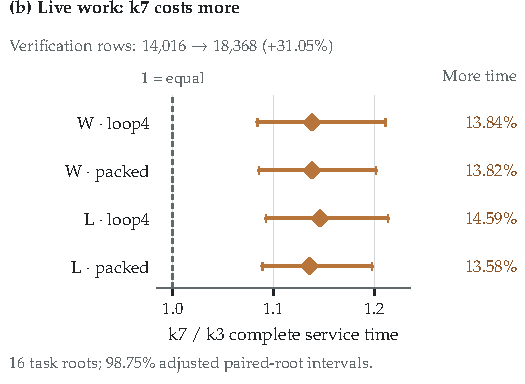
\includegraphics[width=.493\textwidth]{figures/width_live.pdf}
\caption{Equal-work efficiency and live workload. (a) One $q=8$ call versus two $q=4$ calls from the same state, using eight known tokens and all eight full outputs. Diamonds and percentages summarize total operation time; faint points retain all four origin ratios (one APPS, three GSM8K). (b) Four fixed-method $k=7$/$k=3$ service ratios from the separate 16-root live panel, with 98.75\% adjusted intervals; percentages denote increases. D4 is fixed; no contemporaneous M is timed.}
\label{fig:width}
\end{figure*}

Across the four development origins, one $q=8$ operation uses 3.94\%--11.91\% less aggregate time than two $q=4$ operations in the four RTX cells (Fig.~\ref{fig:width}a). Individual origin ratios remain visible, including the loop4-crossing origin above 1. The separate A5000 live pilot is reported in Supplement~S4.

In live generation, k7 reduces cycles from 3,504 to 2,296 per arm but increases verification rows from 14,016 to 18,368 for the same 11,472 emitted tokens. Acceptance among inspected proposals is 87.47\% and 87.93\%; acceptance among all proposals is 75.42\% and 56.94\%. The separate proposal accounts in the supplement distinguish actual mismatches from unconsumed suffixes.

All four complete-service width comparisons favor k3 by the ratios shown in Fig.~\ref{fig:width}b. For LOCAL-packed, $k=7$ adds 24.897\,s over 128 requests: verification adds 13.567\,s, draft proposal adds 13.224\,s, and draft synchronization saves 2.792\,s. Output copying contributes 0.252\,s; the remaining work closes the balance. Supplementary Fig.~S1 and Table~S6 preserve the decomposition and all eight arms.

The complete cost can be written as
\begin{equation}
 T_{\mathrm{spec}}=T_{\mathrm{target}}+T_{\mathrm{draft}}+T_{\mathrm{state/output/host}},
 \label{eq:cost}
\end{equation}
with disjoint intervals and a reconciled residual. Wider execution reduces some per-row cost, while longer proposals alter the total rows and consumed fraction. The evaluated live workload uses k3 as its effective fixed configuration; q8 remains a supported parallel execution capability with its own equal-work evidence.
